\chapter{Used datasets}
\section{Overview of experimental data}

In order to compare the selected libraries and to show examples, it was necessary to select experimental data that can be used as a reference point. For this purpose, one binary classification and one regression dataset was selected.

\subsection{Classification data}
	
	 The classification task was carried out using complete ''\textit{Wisconsin Diagnostic Breast Cancer}'' from November 1995, containing data about cancer tumors. The dataset was created by William H. Wolberg PhDm W. Nick Street and Olvi L. Mangasarian from the University of Wisconsin \cite{wisconsin}. It is available for download from the repository of the University of California \cite{Dua:2019}, and has the following structure:
	 
	\begin{enumerate}
		\item [1)] ID - identification number of a pacient;
		\item [2)] Diagnosis [\textit{Malignant - M} / \textit{Benign - B}] - tumor type, \textbf{response variable};
		\item [3)] Classification data:
			\begin{enumerate}
				\item [a)] \textit{Radius};
				\item [b)] \textit{Texture};
				\item [c)] \textit{Perimeter};
				\item [d)] \textit{Area};
				\item [e)] \textit{Smoothness} - described as local differences in tumor radius;
				\item [f)] \textit{Compactness} - used to determine the stadium of the tumor;
				\item [g)] \textit{Concavity};
				\item [h)] \textit{Concave points};
				\item [i)] \textit{Symmetry} - helpful in evaluation of the spread characteristics;
				\item [j)] \textit{Fractal dimention (,,coastline approximation'' - 1)} - describes the complexity of nerve cells, helping to determine whether cells exhibit cancerous mutations.
			\end{enumerate}
	\end{enumerate}
	
	For each of the variables above, the data contain an average, standard deviation, and average of three highest observations, and are organized sequentially, starting from set of averages. All variables have continuous character. There is also a reduced version of the data containing only the averages set, available as an attachment to this handbook \cite{biostatisticsJMP}.
	
\subsection{Regression data}

	For the demonstation purposes of regression task, the ''IronGlutathione'' dataset attached to this handbook \cite{biostatisticsJMP} was selected. It describes the connection between iron content and glutathione transferase enzyme in human body. It was created in 2012, and contains 90 observations of following 10 variables:  
	
	\begin{enumerate}
		\item \textit{Age};
		\item \textit{Gender};
		\item \textit{Alpha GST (ng/L)} - glutatione transferase type $\alpha$ content;
		\item \textit{pi GST (mg/L)} - glutatione transferase type  $\pi$ content;
		\item \textit{transferrin (mg/mL)};
		\item \textit{sTfR (mg/mL)} - solvable transferin receptor content;
		\item \textit{Iron (mg/dL)};
		\item \textit{TIBC (mg/dL)} - total capacity of iron bonding;
		\item \textit{\%ISAF (Iron / TIBC)} - transferin saturation coefficient;
		\item \textit{Ferritin (ng/dL)};
	\end{enumerate} 
	
	\textit{Ferritin (ng/dL)} was selected as a response variable.
	
\section{Data characteristics}

	During the process of learning by the model, one of the most crucial steps is to familiarize with the dataset and analyze the distribution of the regressors. JMP Pro \cite{jmp} was selected as the software for this purpose.

	\subsection{Classification data}
	\subsubsection{Predictor and response distribution analysis}
		
	The analysis was started by characterising the \textit{Diagnosis} variable. Figure \ref{fig:diagnosisdistribution} shows the histogram and table describing the number of observations in each class and the probability of an observation to belong to each of them. The data contains 357 observations of benign tumor with probability of $\approx$ 62.7\%, and 212 malignant tumors with probability of $\approx$ 37.3\%.
		
	Based on produced histograms, it was determined that majority of the predictors have right-skewed distribution and contain outliers, as shown on the attached box plots from fig. \ref{fig:variabledistribution}. \textit{Mean Largest Concave Points} was an exception for despite having lighly skewed distribution, it contains no outliers. Based on this information, in order to properly teach the model, the data needed to be cleaned and normalized.
	
	\begin{figure}[!ht]
		\centering
		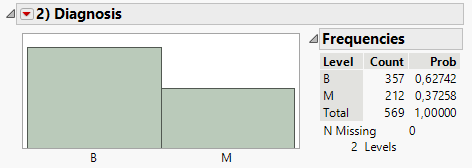
\includegraphics[width=0.6\linewidth]{Rysunki/Rozdzial2/diagnosis_distribution}
		\caption{Response distribution.}
		\label{fig:diagnosisdistribution}
	\end{figure}
	
	\begin{figure}[!ht]
		\centering
		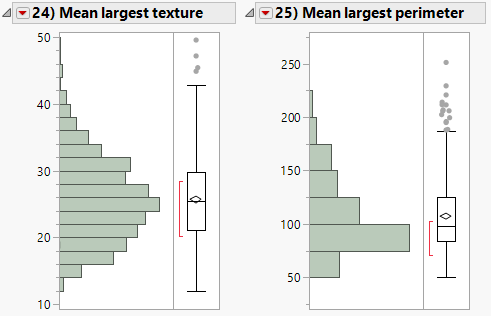
\includegraphics[width=0.6\linewidth]{Rysunki/Rozdzial2/variable_distribution}
		\caption{Predictors distribution sample.}
		\label{fig:variabledistribution}
	\end{figure}
	
	
	\subsubsection{Cleaning and normalizing the data}
	
	The full dataset consists of 569 observations, with 13 missing values for \textit{Std err concave points}, which were filled with the average of other values from this column. Outliers and distribution skewedness proved to be the main problem. Box plots were used to analyze and identify observations with outlying values, where Y axis described the response variable, and X axis the cleaned predictor. Sample graph was shown on fig. \ref{fig:boxgraph}. Due to relatively small size of the dataset, in order to reduce or eliminate the need for excluding observations, the data was first normalized.
	
	\begin{figure}[!ht]
		\centering
		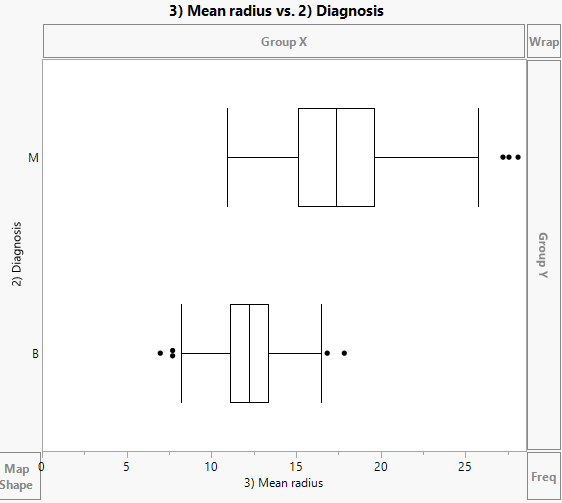
\includegraphics[width=0.7\linewidth]{Rysunki/Rozdzial2/box_graph}
		\caption{Analysis of outliers.}
		\label{fig:boxgraph}
	\end{figure}
	
	Logarithmic transformation was used as a first approach to the normalization task for every predictor. In comparison to the original state, \textit{Mean largest concave points} created a distribution very similar to Gaussian distribution, excluding it from attempts to transform it further. Sample results were shown on fig. \ref{fig:log}. The logarithm proved effective for the following variables:
	
	\begin{enumerate}
		\item \textit{Mean radius};
		\item \textit{Mean texture};
		\item \textit{Mean perimeter},
		\item \textit{Mean area};
		\item \textit{Mean smoothness};
		\item \textit{Mean symmetry};
		\item \textit{Std err texture};
		\item \textit{Std err smoothness};
		\item \textit{Std err compactness};
		\item \textit{Std err concave points};
		\item \textit{Mean largest texture};
		\item \textit{Mean largest smoothness};
		\item \textit{Mean largest compactness}.
	\end{enumerate}

	\begin{figure}[!ht]
		\centering
		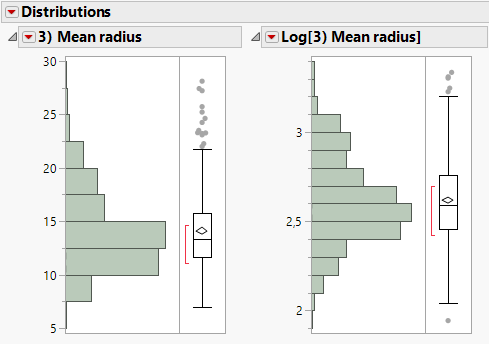
\includegraphics[width=0.7\linewidth]{Rysunki/Rozdzial3/log}
		\caption{Comparison of distributions before and after the logarithmic transformation.}
		\label{fig:log}
	\end{figure}

	Next step was to use cube root transformation on each of the remaining variables, due to its effectiveness on right-skewed data. Figure \ref{fig:cuberoot} shows the achieved results for \textit{Mean concavity}. The transformation was applied to following predictors:
	
	\begin{enumerate}
		\item \textit{Mean compactness};
		\item \textit{Mean concavity};
		\item \textit{Mean concave points};
		\item \textit{Std err concavity};
		\item \textit{Mean largest radius};
		\item \textit{Mean largest perimeter};
		\item \textit{Mean largest concavity};
		\item \textit{Mean largest symmetry}.
	\end{enumerate} 

\begin{figure}[!ht]
	\centering
	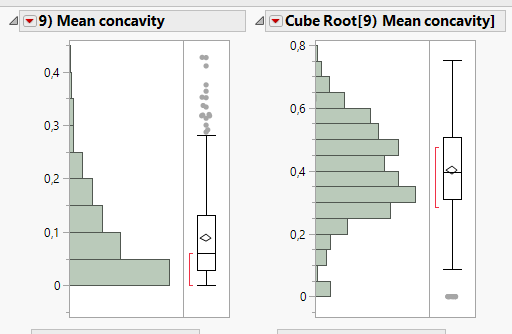
\includegraphics[width=0.7\linewidth]{Rysunki/Rozdzial3/cube_root}
	\caption{Comparison of distributions before and after the cube root transformation.}
	\label{fig:cuberoot}
\end{figure}

	Inverse Arrhenius transformation was used as the last resort. It takes root in the Arrhenius formula describing energy of chemical reaction activation as \ref{eq_arr} \cite{arr}:
	
	\begin{equation}
		\ln k = \ln A - \frac{E_a}{RT}
		\label{eq_arr}
	\end{equation}

	where: 
	\begin{itemize}
		\item $k$ - constant chemical reactivity coefficient;
		\item $A$ - frequency coefficient;
		\item $E_a$ - reaction activation energy;
		\item $R$ - perfect gas constant;
		\item $T$ - reaction temperature in Kelvins;
	\end{itemize}
	
	Sadly, part of the modified variables maintained partial right-skewed distribution, however other available transformations, such as square root, square power, $\log(x+1)$, decimal logarithm, power function, and exponential function provided similar or worse effect. Example result is shown on fig. \ref{fig:arrhenius}. The Inverse Arrhenius transformation was applied to following predictors:
	
	\begin{enumerate}
		\item \textit{Mean fractal dimension};
		\item \textit{Std err radius};
		\item \textit{Std err perimeter};
		\item \textit{Std err area};
		\item \textit{Std err symmetry};
		\item \textit{Std err fractal dimension};
		\item \textit{Mean largest area};
		\item \textit{Mean largest fractal dimension}.
	\end{enumerate}
	
	\begin{figure}[!ht]
		\centering
		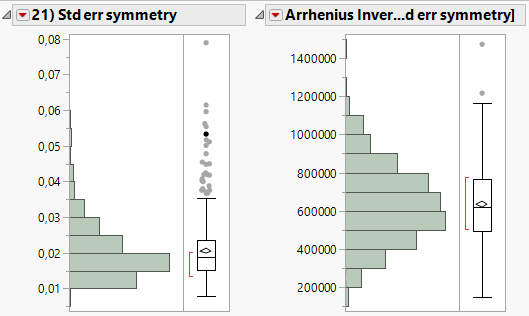
\includegraphics[width=0.7\linewidth]{Rysunki/Rozdzial3/arrhenius}
		\caption{Comparison of the distribution before and after inverse Arrhenius transformation.}
		\label{fig:arrhenius}
	\end{figure}
	
	Due to very small amount of observations, outliers were kept to prevent data loss and further changes in distributions. In order to make the data compatibile with used libraries, the result variable was recoded from using characters to numbers: 1 for malignant and 0 for benign tumor;
	
	Further analysis aimed to exclude highly correlated predictors. This was accomplished via scatterplot matrix, resulting in the exclusion of following variables from the learning process:
	
	\begin{enumerate}
		\item \textit{Log mean perimeter};
		\item \textit{Log mean area};
		\item \textit{Log mean symmetry};
		\item \textit{Arrhenius inverse std err perimeter};
		\item \textit{Arrhenius inverse std err area};
		\item \textit{Cube root std err concavity};
		\item \textit{Cube root mean largest perimeter};
		\item \textit{Log mean largest compactness};
		\item \textit{Cube root mean largest concavity};
		\item \textit{Mean largest concave points};
		\item \textit{Cube root mean largest radius};
		\item \textit{Cube root mean concave points};
		\item \textit{Cube root mean concavity};
		\item \textit{Log std err compactness};
		\item \textit{Log mean largest texture};
		\item \textit{Log mean largest smoothness};
		\item \textit{Cube root mean largest symmetry}.
	\end{enumerate}

	\begin{figure}[!ht]
		\centering
		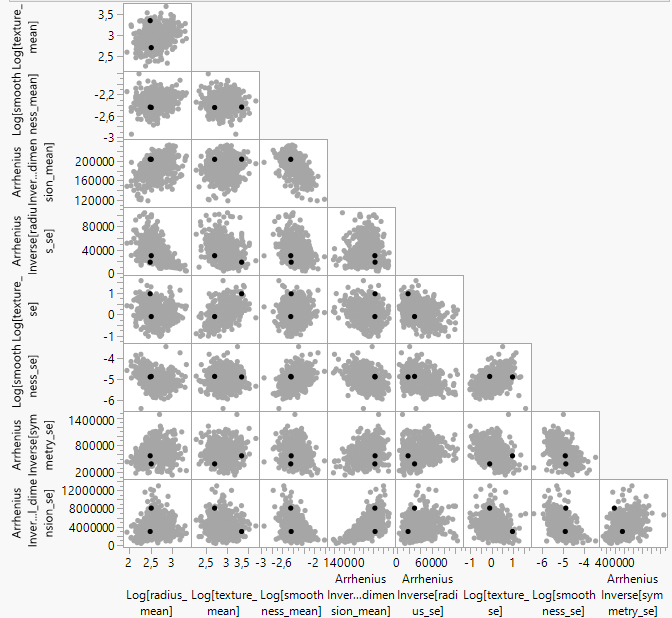
\includegraphics[width=0.9\linewidth]{Rysunki/Rozdzial3/scatter}
		\caption{Scatterplot matrix after removing correlated predictors}
		\label{scatter}
	\end{figure}
	
	Figure \ref{scatter} shows the resulting matrix. After removing correlated variables, the following remained: 
	
	\begin{enumerate}
		\item \textit{Log mean radius};
		\item \textit{Log mean texture};
		\item \textit{Log mean smoothness};
		\item \textit{Arrhenius inverse mean dimension};
		\item \textit{Arrhenius inverse std err radius};
		\item \textit{Log std err texture};
		\item \textit{Log std err smoothness};
		\item \textit{Arrhenius inverse std err symmetry};
		\item \textit{Arrhenius inverse std err dimension}.
	\end{enumerate}

	\subsection{Regression data}	
	\subsubsection{Distribution analysis}
	
	Simiarly to the classification data, the analysis was started from the response variable. It was determined to have highly right-skewed distribution, as shown on fig. \ref{fig:ferritin}.
	
	\begin{figure}[!ht]
		\centering
		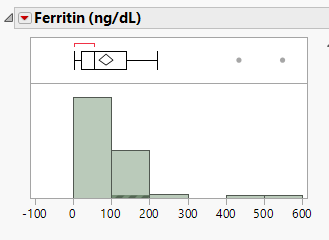
\includegraphics[width=0.5\linewidth]{Rozdzial3/ferritin}
		\caption{Response variable distribution}
		\label{fig:ferritin}
	\end{figure}
	
	Attached box plot shows two outliers. The same problem was spotted for \textit{\%ISAF}, \textit{Iron}, \textit{sTfR}, \textit{Transferrin} and especially \textit{Alpha GST}. Other predictors proved to have distribution close to the Gaussian curve, and not containing any outliers. Figure \ref{fig:decision} shows sample histograms of the predictors.
	
	\begin{figure}[!ht]
		\begin{minipage}{0.40\textwidth}
			\centering
			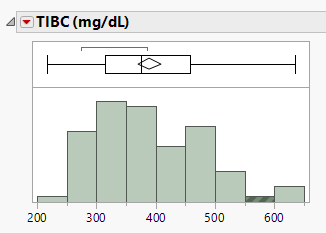
\includegraphics[width=0.9\linewidth]{Rozdzial3/decision}
			\caption{Distribution of TIBC.}
			\label{fig:decision}		
		\end{minipage}%
		\hspace{0.10\textwidth}
		\begin{minipage}{0.40\textwidth}
			\centering
			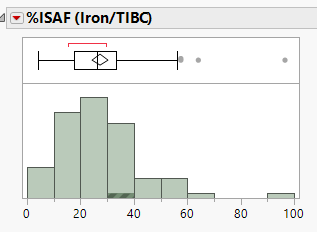
\includegraphics[width=0.9\linewidth]{Rozdzial3/decision1}
			\caption{Distribution of ISAF.}
			\label{fig:decision1}			
		\end{minipage}
	\end{figure}
	
	One variable - \textit{Gender} - has dichotomous character, although it is fairly balanced, with 46.7\% of observations assigned to female (F) class and 53.3\% to male (M) class. Its distribution was showed on fig. \ref{fig:mnf}/
	
	\begin{figure}[!ht]
		\centering
		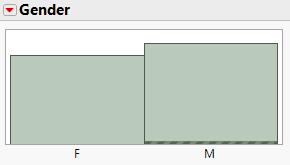
\includegraphics[width=0.6\linewidth]{Rozdzial3/mnf}
		\caption{Distribution of \textit{Gender}.}
		\label{fig:mnf}
	\end{figure}
	
	\subsubsection{Cleaning and normalizing the data}
	
	It was noticed that one observation had missing value for \textit{Ferritin}. Due to only single missing value for 85 observations, the observation without said value was removed. Other things needed to address were normalizing the distribution of some of the predictors and decision in respect to outliers. As previously, normalization came first. Following variables were deemed good as-is:
	
	\begin{enumerate}
		\item \textit{Age};
		\item \textit{Gender};
		\item \textit{TIBC}.
	\end{enumerate}

	For other variables the same three transformations mentioned in section 3.2.1.1 were applied, first of which was using a logarithm. Satisfying result was achieved for predictors:

	\begin{enumerate}
		\item \textit{alpha GST};
		\item \textit{pi GST};
		\item \textit{sTfR};
		\item \textit{Ferritin} (response variable).
	\end{enumerate}

	Figure \ref{fig:log2} shows sample change in distribution.
	
	\begin{figure}[!ht]
		\centering
		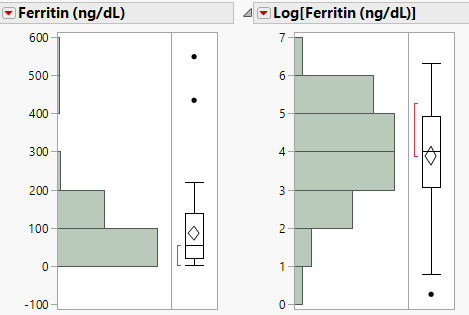
\includegraphics[width=0.6\linewidth]{Rozdzial3/log2}
		\caption{Effect of logarithmic transformation on distribution}
		\label{fig:log2}
	\end{figure}

	Second modification via cube root was successfully used, as shown on fig. \ref{fig:cube2}, for these variables:
	
	\begin{enumerate}
		\item \textit{Transferrin};
		\item \textit{Iron};
		\item \textit{\%ISAF}.
	\end{enumerate}

	\begin{figure}
		\centering
		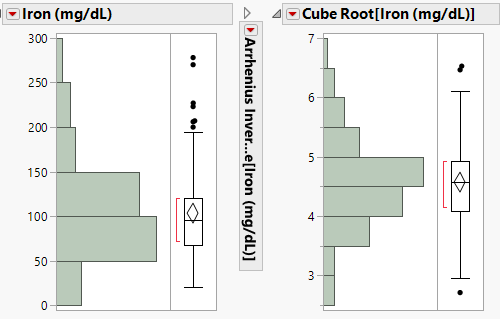
\includegraphics[width=0.6\linewidth]{Rozdzial3/cube2}
		\caption{Cube root distribution normalization}
		\label{fig:cube2}
	\end{figure}

	The inverse Arrhenius transformation proved ineffective for every variable, producing worse effects from the previous methods. Due to low total amount of observations, and relatively few outliers, it was decided that they should be kept for the learning process. To make the data compatibile with used libraries, the \textit{Gender} variable was recoded from characters to numbers: 1 for female, 0 for male.

\section{Models built in JMP}

After the analysis of the datasets, a few models were selected to serve as a reference for practical tests. Sections below present used templates for the models, such as predictors choice chosen based on practical experimentation with JMP machine learning software.

\subsection{Support Vector Machine (SVM)}

This model accepted all variables remaining after the exploration process for learning. A randomized set of observations was used for the validation purpose, in proportions of 80\% learning data and 20\% testing data, using value 1234 as seed for the pseudorandom number generator. \textit{Radial Basis Function} was chosen as the SVM kernel, which is a default choice for this model in JMP environment.

\begin{longtable}{l | c}
	\centering
	Predictor & Learned coefficient \\
	\hline
	\textit{Log mean radius} & 2,6191 \\
	\textit{Log mean texture} & 2,9353 \\
	\textit{Log mean smoothness} & -2,3502 \\
	\textit{Arrhenius inverse mean dimension} & 186640 \\
	\textit{Arrhenius inverse std err radius} & 38170 \\
	\textit{Log std err texture} & 0.1049 \\
	\textit{Log std err smoothness} & -5,0286 \\
	\textit{Arrhenius inverse std err symmetry} & 635100 \\
	\textit{Arrhenius inverse std err dimension} & 4053000 \\
	\caption{Predictors coefficients after learning process.}
	\label{svm:1}
\end{longtable} 

\begin{figure}[!ht]
	\begin{minipage}{0.48\textwidth}
		\centering
		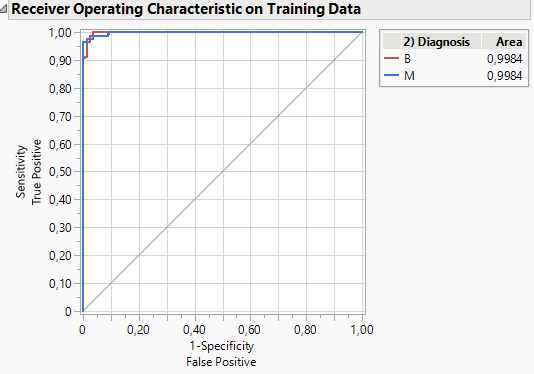
\includegraphics[width=0.98\linewidth]{Rysunki/Rozdzial3/roc_svm1_test}
		\caption{ROC curve for the learning data.}
		\label{fig:rocsvm1test}		
	\end{minipage}%
	\hspace{10pt}
	\begin{minipage}{0.48\textwidth}
		\centering
		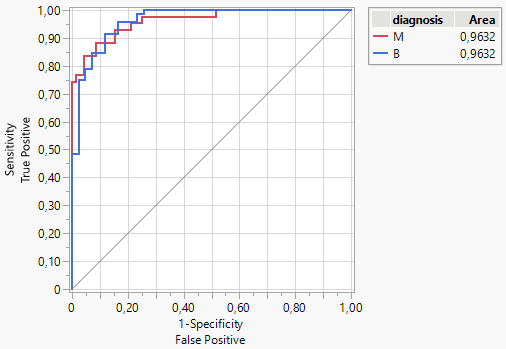
\includegraphics[width=0.98\linewidth]{Rysunki/Rozdzial3/roc_svm1_val}
		\caption{ROC curve for the testing data.}
		\label{fig:rocsvm1val}				
	\end{minipage}	
\end{figure}

The model achieved missclassification rate of 2.64\% for learning data and 9.57\% for testing data. Table \ref{svm:1} shows coefficients determined during learning process for each of the predictors. Figures \ref{fig:rocsvm1test} and \ref{fig:rocsvm1val} show receiver operation characteristic curves for learning and validation data respectively, presenting classification accuracy of 0.9972 for the former and 0.9632 for the latter. 

\subsection{Linear regression}

To determine which predictors have the biggest impact on the response, the p-value was calculated for each of the variables. It was decided that the acceptance threshold should be a p-value equal or below 0.05. Figure \ref{fig:pvalue3} shows a plot for all predictors, and fig. \ref{fig:pvalue4} only for those selected for the learning process.

\begin{figure}[!ht]
	\centering
	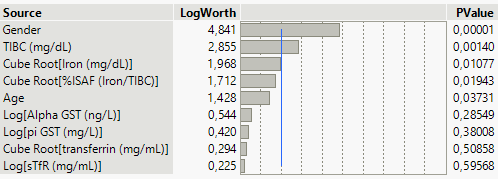
\includegraphics[width=0.6\linewidth]{Rozdzial3/pvalue3}
	\caption{P-value plot for all predictors.}
	\label{fig:pvalue3}
\end{figure}

\begin{figure}[!ht]
	\centering
	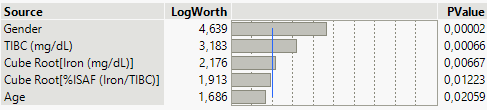
\includegraphics[width=0.7\linewidth]{Rozdzial3/pvalue4}
	\caption{P-value plot for selected predictors.}
	\label{fig:pvalue4}
\end{figure}

Through the process of elimination, the variables mentioned in the table \ref{pvalue} were chosen for the learning process:

\begin{table}[!ht]
	\begin{minipage}{0.48\textwidth}
		\centering
		\begin{tabular}{l|c}
			Predictor & p-value \\
			\hline
			\textit{Gender} & 0.00002 \\
			\textit{TIBC} & 0.00066 \\
			\textit{Cube Root Iron} & 0.00667 \\
			\textit{Cube Root \%ISAF} & 0.01223 \\
			\textit{Age} & 0.02059
		\end{tabular}
		\caption{Selected predictors and their p-value}
		\label{pvalue}
	\end{minipage}%
	\hspace{0.04\textwidth}
	\begin{minipage}{0.48\textwidth}
		\centering
		\begin{tabular}{l|c}
			Predictors & Weight \\
			\hline
			\textit{Intercept} & 8,498959 \\
			\textit{Age} & 0.0201022 \\
			\textit{Gender[F - M]} & -0.959795 \\
			\textit{Cube Root Iron} & 2,9461861 \\
			\textit{TIBC} & -0.014182 \\
			\textit{Cube Root \%ISAF} & -4,356345
		\end{tabular}
		\caption{Weights assigned to the predictors}
		\label{weights}		
	\end{minipage}
\end{table}

As a result of the learning, a model was created with the linear determination coefficient \textit{$R^2$} of 0.4654525, which suggests that the data are moderately well linearly approximable. The table \ref{weights} shows the learned weights for each of the predictors.